\documentclass{beamer}
\usepackage[british,spanish]{babel}
\usepackage[utf8]{inputenc}
\usepackage[british,spanish]{babel}
%usepackage[utf8]{inputenx}

\usepackage{hyperref}
%\hypersetup{colorlinks=false,linkbordercolor=red,linkcolor=green,pdfborderstyle={/S/U/W 1}}

\usepackage{multirow}

\usepackage{textcomp}

\usepackage{listings}
\lstloadlanguages{Ruby}
\usepackage{cancel}

\usepackage{adjustbox}
\usepackage{lstcustom}

\usepackage{amsmath}

\usepackage{color}
\definecolor{light-gray}{gray}{0.80}
\definecolor{lstbackgroundshellcolor}{named}{light-gray}

\usepackage{tikz}
\newcommand*\circled[1]{\tikz[baseline=(char.base)]{
            \node[shape=circle,draw,inner sep=2pt] (char) {#1};}}

\usepackage[normalem]{ulem}

%\usepackage[acronym,xindy,toc]{glossaries}

\usepackage[acronym,xindy,toc]{glossaries}
\makeglossaries
%\usepackage[xindy]{imakeidx}
%\makeindex


\newcommand{\comment}[2]{#2}

\newcommand{\commandinline}[1]{\lstinline[basicstyle=\small\lstfontfamily]{#1}}
\newcommand{\outputcommand}[1]{\color{darkgreen}{#1}}

\graphicspath{ {./images/} }

\title{Storing Data with Amazon S3 and Distributing Data with CloudFront}
%\subtitle[short subtitle]{long subtitle}
\author[C. Cuenca, F. Quintana]{Carmelo Cuenca-Hernández and Francisca Quintana-Domínguez}
%\institute{Escuela Universitaria de Informática}
%\date[04/2013]{Abril - 2013}
\date{}
\titlegraphic{
\includegraphics[width=0.5 \textwidth]{./images/logo_ulpgc_version_horizontal_rgb.eps}}


\pgfdeclareimage[width=2.0\baselineskip]{ulpgc-logo}{images/logosimbolo_secundario_version_vertical}
\setbeamertemplate{footline}{\raisebox{-2ex}{\pgfuseimage{ulpgc-logo}}
  \usebeamerfont{date in head/foot}\insertshortdate{}\hfill
  \usebeamertemplate{navigation symbols}\hfill
  \insertframenumber{}/\inserttotalframenumber}
\setbeamertemplate{sidebar right}{}


\usetheme{Antibes}
%\usetheme{Berlin}

%\usetheme{Warsaw}
%\usecolortheme{albatross}

\selectlanguage{british}



\begin{document}

%
\includegraphics[width= 1.0 \textwidth]{logos3.eps}
\begin{frame}
	\titlepage
\end{frame}


\section*{Outline}
\begin{frame}[fragile, allowframebreaks]
  \frametitle{Outline}
  %\tableofcontents%[part=1,pausesections]
  \tableofcontents[currentsection,currentsubsection, sectionstyle=show] 
  %\tableofcontents[currentsection,sectionstyle=show,hideothersubsections]
\end{frame}

%%%%%%%%%%%%%%%%%%%%%%%%%%%%%%%%%%%%%%%%%%%%%%%%%%%%%%%%%%%%%%%%%%%%%%%%%%%%%%
%\newacronym{<label>}{<abbrv>}{<full>}
%\glsreset{<label>}
%\glsresetall
%\acrlong{<label>}
%\acrfull{<label>}
%\acrshort{<label>}
%\input{../glossary}

\newacronym{acl}{ACL}{Access Control List}
\newacronym{api}{API}{Application Programming Interface}
\newacronym{aws}{AWS}{Amazon Web Services}
\newacronym{cli}{CLI}{Command Line Interface}
\newacronym{css}{CSS}{cascading style sheets}
\newacronym{ebs}{EBS}{Elastic Block StoAWS Identity an Access Managementrage}
\newacronym{ec2}{EC2}{Amazon Elastic Compute Cloud}
\newacronym{elb}{ELB}{Elastic Load Balancing}
\newacronym{iam}{IAM}{Identity Access Management}
\newacronym{ror}{RoR}{{\href{http://rubyonrails.org/}{Ruby on Rails}}}
\newacronym{rds}{RDS}{Relational Database Service}
\newacronym{rvm}{RVM}{{\href{https://rvm.io/}{Ruby Version Manager}}}
\newacronym{s3}{S3}{Simple Storage Service}
\newacronym{sqs}{SQS}{Amazon Simple Queue Service}
%%%%%%%%%%%%%%%%%%%%%%%%%%%%%%%%%%%%%%%%%%%%%%%%%%%%%%%%%%%%%%%%%%%%%%%%%%%%%%
\section{Storing Data with Amazon S3}
\begin{frame}[fragile, allowframebreaks]
\frametitle{Storing Data with Amazon S3}
\begin{itemize}
 \item \acrfull{s3} is an Internet-scale data storage service
 \item \acrshort{s3} lets you store your data in containers called \textbf{buckets}
  \begin{itemize}
 \item A bucket is a named storage entity attached to a particular \acrshort{aws} account. You can create up to 100 buckets in your \acrshort{aws} account
 \item The bucket names must be globally unique, so you’ll have to choose with care and keep on trying until you find available names
 \item Buckets are used to group any number of S3 objects
\end{itemize}
 \item You can store any type of data you like in \acrshort{s3} (HTML pages, CSS style sheets, or C source code, or binary files such as JPEG images, tar
backup files, or even encrypted data (you can encrypt sensitive data before storing
it in \acrshort{s3}, if you’d like)
 \item \acrshort{s3} is ideal for storing web data
 \item Each \acrshort{s3} object has its own URL and \acrshort{s3} can handle a very high request rate
\item \acrshort{s3} can store objects of up to 5GB in size

\end{itemize}
\end{frame}
%%%%%%%%%%%%%%%%%%%%%%%%%%%%%%%%%%%%%%%%%%%%%%%%%%%%%%%%%%%%%%%%%%%%%%%%%%%%%

\begin{frame}[fragile]
\frametitle{\acrshort{s3} Object Identification}
\begin{itemize}
\item Every \acrshort{s3} object has a unique URL formed by concatenating these components:
\begin{enumerate}
\item protocol (\texttt{http://} or \texttt{https://})
\item bucket name ending with ``.''
\item S3 endpoint (\texttt{s3.amazonaws.com})
\item object key starting with ``/''
\end{enumerate}
\end{itemize}

\end{frame}

%%%%%%%%%%%%%%%%%%%%%%%%%%%%%%%%%%%%%%%%%%%%%%%%%%%%%%%%%%%%%%%%%%%%%%%%%%%%%%
%%%%%%%%%%%%%%%%%%%%%%%%%%%%%%%%%%%%%%%%%%%%%%%%%%%%%%%%%%%%%%%%%%%%%%%%%%%%%%

\begin{frame}[fragile]
\frametitle{Access to S3 bucket and object}
\begin{itemize}
\item Access to each \acrshort{s3} bucket and object is regulated by an \acrfull{acl}
\item An \acrshort{acl} contains a series of up to 100 grants, with each grant consisting of a grantee
and a permission

\scalebox{0.75}{
\begin{tabular}{|l|p{5cm}|p{5cm}|} \hline
Permission & When applied to a bucket & When applied to an object\\ \hline
READ & Permission to list the contents of the bucket & Permission to read the object or its metadata\\ \hline
WRITE & Permission to create, replace, or delete any object in the bucket & Unsupported for objects\\ \hline
READ\_ACP & Permission to read the bucket’s ACL & Permission to read the object’s ACL\\ \hline
WRITE\_ACP & Permission to overwrite the bucket’s ACL & Permission to overwrite the object’s ACL\\ \hline
FULL\_CONTROL & All of the above & All of the above\\ \hline
\end{tabular} 
}
\end{itemize}

\end{frame}

%%%%%%%%%%%%%%%%%%%%%%%%%%%%%%%%%%%%%%%%%%%%%%%%%%%%%%%%%%%%%%%%%%%%%%%%%%%%%%
%%%%%%%%%%%%%%%%%%%%%%%%%%%%%%%%%%%%%%%%%%%%%%%%%%%%%%%%%%%%%%%%%%%%%%%%%%%%%%

\begin{frame}[fragile]
\frametitle{S3 Pricing Model}
\begin{itemize}
\item Your \acrshort{s3} usage is charged in three dimensions:
\begin{itemize}
\item amount of data stored
\item amount of data transferred in and out of \acrshort{s3}
\item the number of requests made to \acrshort{s3}
\end{itemize}
\end{itemize}

\begin{alertblock}{Warning}
You need to keep in mind that the meter is always running! If you write a program
to poll one of your \acrshort{s3} buckets every second (a LIST request) you’ll be spending
86 cents every day, whether there’s anything new in the bucket or otherwise. You
should also check your loop terminating conditions with extreme care. It’s better
to avoid writing an infinite loop which costs you money with every iteration
\end{alertblock}

\end{frame}
%%%%%%%%%%%%%%%%%%%%%%%%%%%%%%%%%%%%%%%%%%%%%%%%%%%%%%%%%%%%%%%%%%%%%%%%%%%%%%
%%%%%%%%%%%%%%%%%%%%%%%%%%%%%%%%%%%%%%%%%%%%%%%%%%%%%%%%%%%%%%%%%%%%%%%%%%%%%%
\section{S3 AWS Management Console}
%%%%%%%%%%%%%%%%%%%%%%%%%%%%%%%%%%%%%%%%%%%%%%%%%%%%%%%%%%%%%%%%%%%%%%%%%%%%%%
\begin{frame}[fragile]
\frametitle{S3 AWS Management Console}
\begin{itemize}
\item With the AWS Management Console you can easily manage Amazon S3 buckets and objects. You can create buckets, upload objects, and manage all aspects of your Amazon S3 resources
\end{itemize}

\begin{columns}
 \column{0.33 \textwidth}
 \begin{itemize}
 \item Create Buckets
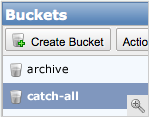
\includegraphics[width= 0.75 \textwidth]{console_thumb_s3_01.png}
 \end{itemize}
\column{0.33 \textwidth}
\begin{itemize}
 \item Upload Files
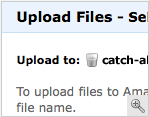
\includegraphics[width= 0.75 \textwidth]{console_thumb_s3_02.png}
 \end{itemize}
\column{0.33 \textwidth}
\begin{itemize}
 \item Manage Your Resources
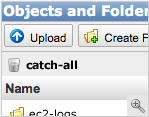
\includegraphics[width= 0.75 \textwidth]{console_thumb_s3_03.png}
 \end{itemize}
\end{columns}

\end{frame}
%%%%%%%%%%%%%%%%%%%%%%%%%%%%%%%%%%%%%%%%%%%%%%%%%%%%%%%%%%%%%%%%%%%%%%%%%%%%%%
\section{Setup and Running AWS API}
\begin{frame}[fragile, allowframebreaks]
\frametitle{Setup and Running AWS API}
\begin{itemize}
  \item \url{http://aws.amazon.com/documentation/sdkforruby/}
  \item  Install the AWS Ruby gem

\lstset{language=shell}
\begin{lstlisting}[escapechar=!]
$  gem install aws-sdk
\end{lstlisting}

  \item Run the Samples
  \begin{itemize}
 


    \item Now that you’ve installed the gem, you can run the samples, which you can find in our GitHub repository:

\lstset{language=shell}
\begin{lstlisting}[escapechar=!]
  $ git clone https://github.com/aws/aws-sdk-ruby
  $ cd aws-sdk-ruby/samples/
\end{lstlisting}

  \item You need to provide your \acrshort{aws} security credentials and choose a default region
    \begin{itemize}
    
      \item Hardcode ?
\begin{lstlisting}[escapechar=!]
     AWS.config(access_key_id: '...', secret_access_key: '...', region: 'us-west-2')
\end{lstlisting}
      \item Or you can also specify these values via `ENV`:
\lstset{language=shell}
\begin{lstlisting}[escapechar=!]
  $ export AWS_ACCESS_KEY_ID='...'
  $ export AWS_SECRET_ACCESS_KEY='...'
  $ export AWS_REGION='us-west-2'
\end{lstlisting}


      \item Or you can reate a file named \texttt{config.yml} in the samples directory as follows:
\lstset{language=Ruby, style=eclipse}
\begin{lstlisting}[escapechar=!]
      # Fill in your AWS Access Key ID and Secret Access Key
      # http://aws.amazon.com/security-credentials
      access_key_id: REPLACE_WITH_ACCESS_KEY_ID
      secret_access_key: REPLACE_WITH_SECRET_ACCESS_KEY
\end{lstlisting}
    \end{itemize}
  \item The subdirectories of the samples directory contain several code samples that you can run
  \end{itemize}
\end{itemize}

\end{frame}
%%%%%%%%%%%%%%%%%%%%%%%%%%%%%%%%%%%%%%%%%%%%%%%%%%%%%%%%%%%%%%%%%%%%%%%%%%%%%%
%%%%%%%%%%%%%%%%%%%%%%%%%%%%%%%%%%%%%%%%%%%%%%%%%%%%%%%%%%%%%%%%%%%%%%%%%%%%%%
\section{Programming S3}
\subsection{Creating a S3 bucket}
\begin{frame}[fragile, allowframebreaks]
\frametitle{Creating a S3 bucket}
\begin{itemize}

\item Set up aws project directory
\lstset{language=shell, escapechar=!}
\begin{lstlisting}[escapechar=!]
$ mkdir ~/ruby_projects
$ mkdir ~/ruby_projects/aws_app
$ echo "2.0.0" > ~/ruby_projects/aws_app/.ruby-version
$ echo "aws_app" > ~/ruby_projects/aws_app/.ruby-gemset
$ cd ~/ruby_projects/aws_app
\end{lstlisting}

\item \texttt{aws\_app/config.yml}
\lstset{language=shell, escapechar=!}
\begin{lstlisting}[escapechar=!]
#
# aws_app/config.yml
#
# Fill in your AWS Access Key ID and Secret Access Key
# http://aws.amazon.com/security-credentials
               
access_key_id: YOUR_ACCESS_KEY_ID
secret_access_key: YOUR_SECRET_ACCESS_KEY
\end{lstlisting}

\item \texttt{aws\_app/config.rb}
\lstset{language=Ruby, style=eclipse}
\begin{lstlisting}[escapechar=$]
# Copyright 2011-2013 Amazon.com, Inc. or its affiliates. All Rights Reserved.
#
# Licensed under the Apache License, Version 2.0 (the "License"). You
# may not use this file except in compliance with the License. A copy of
# the License is located at
#
#     http://aws.amazon.com/apache2.0/
#
# or in the "license" file accompanying this file. This file is
# distributed on an "AS IS" BASIS, WITHOUT WARRANTIES OR CONDITIONS OF
# ANY KIND, either express or implied. See the License for the specific
# language governing permissions and limitations under the License.

require 'rubygems'
require 'yaml'
require 'aws-sdk'

config_file = File.join(File.dirname(__FILE__),
                        "config.yml")
unless File.exist?(config_file)
  puts <<END
To run the samples, put your credentials in config.yml as follows:

access_key_id: YOUR_ACCESS_KEY_ID
secret_access_key: YOUR_SECRET_ACCESS_KEY

END
  exit 1
end

config = YAML.load(File.read(config_file))

unless config.kind_of?(Hash)
  puts <<END
config.yml is formatted incorrectly.  Please use the following format:

access_key_id: YOUR_ACCESS_KEY_ID
secret_access_key: YOUR_SECRET_ACCESS_KEY

END
  exit 1
end

AWS.config(config)
\end{lstlisting}

\item \texttt{aws\_app/s3/s3/book.inc.rb}
\lstset{language=Ruby, style=eclipse}
\begin{lstlisting}[escapechar=$]
#
# aws_app/s3/book.inc.rb
#
# This file is required by some *.rb files
# It defines default constant value

BOOK_BUCKET = :developing_cloud_application_bucket # $\circled{1}$
\end{lstlisting}

\item \texttt{aws\_app/s3/create\_bucket.rb}
\lstset{language=Ruby, style=eclipse}
\begin{lstlisting}[escapechar=$]
#
# aws_app/s3/create_bucket.rb
#
# Usage: ruby create_bucket.rb [<bucket_name>]
# When bucket_name is not used
# Then name bucket BOOK_BUCKET defined in book.inc.rb file is used
#

require File.expand_path("#{File.dirname(__FILE__)}/../config")
require File.expand_path("#{File.dirname(__FILE__)}/book.inc")

if ARGV.size > 1
  puts "Usage: #{__FILE__} [<BUCKET_NAME>]"
  exit 1
end

bucket_name =  ARGV.size != 1 ? BOOK_BUCKET :  ARGV[0]

# get an instance of the s3 interface using the default configuration
s3 = AWS::S3.new

begin
  bucket = s3.buckets.create bucket_name
  puts "#{bucket.name} bucket created"
rescue Exception => e
  puts e.message
end
\end{lstlisting}

\item Run the code
\lstset{language=shell}
\begin{lstlisting}[escapechar=!]
  $ ruby s3/create_bucket.rb
  $ ruby s3/create_bucket.rb obama
  $ ruby s3/create_bucket.rb <my-bucket-name>
\end{lstlisting}

\end{itemize}
\end{frame}
%%%%%%%%%%%%%%%%%%%%%%%%%%%%%%%%%%%%%%%%%%%%%%%%%%%%%%%%%%%%%%%%%%%%%%%%%%%%%%
\subsection{Listing your S3 buckets}
\begin{frame}[fragile, allowframebreaks]
\frametitle{Listing your S3 buckets}
\begin{itemize}
\item Here is how to list your S3 buckets (\texttt{list\_buckets.rb})

\lstset{language=Ruby, style=eclipse}
\begin{lstlisting}[escapechar=!]
#
# aws_app/s3/list_buckets.rb
#
# Usage: ruby list_buckets.rb
#

require File.expand_path("#{File.dirname(__FILE__)}/../config")

# get an instance of the S3 interface using the default configuration
s3 = AWS::S3.new

s3.buckets.each{|bucket| puts bucket.name}
\end{lstlisting}

\item Run the code
\lstset{language=shell}
\begin{lstlisting}[escapechar=!]
$ ruby s3/list_buckets.rb
!\outputcommand{carmelo.cuenca\\
developing\_cloud\_application\_bucket\\
francisca.quintana}!
\end{lstlisting}

\item This is a simple yet powerful piece of code. We established a connection to S3, retrieved a list of buckets, iterate over the result, and printed the name of each bucket on a line of its own
\end{itemize}
\end{frame}
%%%%%%%%%%%%%%%%%%%%%%%%%%%%%%%%%%%%%%%%%%%%%%%%%%%%%%%%%%%%%%%%%%%%%%%%%%%%%%
%%%%%%%%%%%%%%%%%%%%%%%%%%%%%%%%%%%%%%%%%%%%%%%%%%%%%%%%%%%%%%%%%%%%%%%%%%%%%%
\subsection{Bucket Listing as a Web Page}
\begin{frame}[fragile, allowframebreaks]
\frametitle{Bucket Listing as a Web Page}
\begin{itemize}
\item Install the minimalistic ``Sinatra'' framework
\lstset{language=shell}
\begin{lstlisting}[escapechar=!]
$ gem install sinatra
\end{lstlisting}


\item There are numerous template engines available; \texttt{Erb}, \texttt{Haml}, and \texttt{Erubis} are
just a few. We’ll use \texttt{Erb} for our templates as it’s fairly ubiquitous in the Ruby community these days, although any mature engine will do just fine as the usage is essentially the same in all cases

\item Write the template view file \texttt{aws\_app/views/s3/list\_buckets.html.erb}

\lstset{language=Ruby, style=eclipse}
\begin{lstlisting}[escapechar=?]
<!DOCTYPE html>
<html>
<head>
  <title><%= @output_title %></title>
</head>
<body>
  <div>
    <h1><%= @output_title %></h1>
    <p><%= @output_message %></p>
    <ul>
      <% @s3.buckets.each do |bucket| %>
        <li> <%= bucket.name %> </li>
      <% end %>
    </ul>
  </div>
</body>
</html>
\end{lstlisting}


\item Write the server code to server the page
\lstset{language=Ruby, style=eclipse}
\begin{lstlisting}[escapechar=!]
#
# aws_app/server.rb
#
require 'sinatra'
require File.expand_path("#{File.dirname(__FILE__)}/config")

get '/s3/list_buckets' do
  # get an instance of the S3 interface using the default configuration
  @s3 = AWS::S3.new
  @output_title = 'Expert in Virtualization and Cloud Computing - List of S3 buckets'
  @output_message = 'A simple HTML list of your S3 buckets'
  erb :'/s3/list_buckets.html'
end
\end{lstlisting}

\item Curl to url \url{http://localhost:4567/s3/list_buckets}
\end{itemize}
\end{frame}
%%%%%%%%%%%%%%%%%%%%%%%%%%%%%%%%%%%%%%%%%%%%%%%%%%%%%%%%%%%%%%%%%%%%%%%%%%%%%%
\subsection{Listing Objects in a Bucket}
\begin{frame}[fragile,allowframebreaks]
\frametitle{Listing Objects in a Bucket}
\begin{itemize}
 \item We list all the objects within the first bucket we created (using the constant \texttt{BOOK\_BUCKET})

\lstset{language=Ruby, style=eclipse}
\begin{lstlisting}
#
# aws_app/s3/list_bucket_objects.rb
#
# Usage: ruby list_bucket_objects.rb [<bucket_name>]
# When bucket_name is not used
# Then name bucket BOOK_BUCKET defined in book.inc.rb file is used
#

require File.expand_path("#{File.dirname(__FILE__)}/../config")
require File.expand_path("#{File.dirname(__FILE__)}/book.inc")

# access to bucket in ARGV[0] or BOOK_BUCKET

if ARGV.size > 1
  puts "Usage: #{__FILE__} [<BUCKET_NAME>]"
  exit 1
end
bucket_name =  ARGV.size != 1 ? BOOK_BUCKET :  ARGV[0]

begin
  # get an instance of the S3 interface using the default configuration
  s3 = AWS::S3.new
  bucket = s3.buckets[bucket_name]
  bucket.objects.each{|obj| puts obj.key }
rescue Exception => e
  puts e.message
end
\end{lstlisting}
\end{itemize}

\end{frame}
%%%%%%%%%%%%%%%%%%%%%%%%%%%%%%%%%%%%%%%%%%%%%%%%%%%%%%%%%%%%%%%%%%%%%%%%%%%%%%
\begin{frame}[fragile,allowframebreaks]
\frametitle{What happens with metadata?}
\begin{itemize}
 \item We list all the objects within a bucket we some metadata (using the constant \texttt{BOOK\_BUCKET} as default)

\lstset{language=Ruby, style=eclipse}
\begin{lstlisting}
#
# aws_app/s3/list_bucket_objects_raw.rb
#
# Usage: ruby list_bucket_objects_raw.rb [<bucket_name>]
# When bucket_name is not used
# Then name bucket BOOK_BUCKET defined in book.inc.rb file is used
#

require File.expand_path("#{File.dirname(__FILE__)}/../config")
require File.expand_path("#{File.dirname(__FILE__)}/book.inc")

# access to bucket in ARGV[0] or BOOK_BUCKET

if ARGV.size > 1
  puts "Usage: #{__FILE__} [<BUCKET_NAME>]"
  exit 1
end
bucket_name =  ARGV.size != 1 ? BOOK_BUCKET :  ARGV[0]

begin
  # get an instance of the S3 interface using the default configuration
  s3 = AWS::S3.new

  bucket = s3.buckets[bucket_name]
  bucket.objects.each do |obj|
    puts obj.key
    puts obj.head.each {|key, value| puts "  #{key}: #{value}"}
  end
rescue Exception => e
  puts e.message
end
\end{lstlisting}
\end{itemize}

\end{frame}

%%%%%%%%%%%%%%%%%%%%%%%%%%%%%%%%%%%%%%%%%%%%%%%%%%%%%%%%%%%%%%%%%%%%%%%%%%%%%%
\begin{frame}[fragile,allowframebreaks]
\frametitle{Listing Objects in a Bucket as a Web Page}
\begin{itemize}
 \item We first write the method \texttt{get\_bucket\_objects} which simply calls \texttt{list\_objects} again and again until S3 says than are no more objects to return

\lstset{language=Ruby, style=eclipse}
\begin{lstlisting}[escapechar=!]
#
# aws_app/book.inc.rb
#
# This file is required by some *.rb files
# It defines default constant value
# and some useful functions
#
BOOK_BUCKET = :developing_cloud_application_bucket
S3_AMAZONAWS_URL = 'https://s3.amazonaws.com'

def get_bucket_objects(s3, bucket_name, prefix = '') #!\circled{1}!
  options = {bucket_name: bucket_name, marker: '', max_keys: 8, prefix: prefix}
  begin
    objects = []
    begin #!\circled{3}!
      response = s3.client.list_objects options #!\circled{4}!
      response.data[:contents].each {|obj| objects << obj} #!\circled{5}!
      is_truncated = response.data[:truncated] #!\circled{6}!
      options[:marker] = objects[-1][:key] if is_truncated #!\circled{7}!
    end while is_truncated
    return objects #!\circled{8}!
  rescue Exception => e
      puts e.message
  end
end
\end{lstlisting}

\begin{itemize}
\item \circled{1} Our function accepts three arguments: an AmazonS3 object, an S3 bucket, and a prefix value that defaults to an empty string.
\item \circled{2} We use a \texttt{do \dots while} loop, so that the body of the loop always runs at least
once
\item \circled{3} Each time we call \texttt{list\_objects}, we pass in a value called \texttt{marker}, The first time it is an empty string. On subsequent loop iterations it is set to the final key returned on the previous iteration
\item \circled{4} If the \texttt{list\_objects} call fails, the function throw an exception
\item \circled{5} We retrieve the Contents array from the body of the response returned to our
\texttt{list\_objects} call, then loop through the values storing each one in the \texttt{objects} array. This array will eventually be our return value.
\item \circled{6} The data returned by a call to \texttt{list\_objects} includes an element named
\texttt{truncated}. If this value is \texttt{true}, the listing is incomplete and
there are more objects to be found. This condition is also used to control the
loop
\item \circled{7} If the list is incomplete, we set the next value ready to begin the next iteration
\item \circled{8} When the loop terminates, the \texttt{objects} array is returned
\end{itemize}



\item The we write the template view file \texttt{aws\_app/views/s3/list\_bucket\_objects.html.erb}
\lstset{language=Ruby, style=eclipse}
\begin{lstlisting}[escapechar=?]
<!DOCTYPE html>
<html>
<head>
  <title><%= @output_title %></title>
</head>
<body>
<div>
  <h1><%= @output_title %></h1>
  <p><%= @output_message %></p>
  <table>
    <thead>
    <tr><th>File</th><th>Size</th></tr>
    </thead>
    <tbody>
    <% @bucket_objects.each do |object| %>
        <tr>
          <td><a href="<%= "#{S3_AMAZONAWS_URL}/#{@bucket_name}/#{object[:key]}" %>"><%= object[:key] %></a></td>
          <td><%= object[:size] %></td>
        </tr>
    <% end if @bucket_objects %>
    </tbody>
  </table>
</div>
</body>
</html>
\end{lstlisting}

\item Next step is to add an entry in file \texttt{server.rb} to
\lstset{language=Ruby, style=eclipse}
\begin{lstlisting}[escapechar=!]
#
# aws_app/server.rb
#
!\vdots!
get '/s3/list_bucket_objects' do
  # get an instance of the S3 interface using the default configuration
  @s3 = AWS::S3.new
  @bucket_name = params[:bucket_name].nil? ? BOOK_BUCKET : params[:bucket_name]
  @output_title = 'Expert in Virtualization and Cloud Computing - List of S3 objects in a bucket'
  @output_message = "A simple HTML table displaying of all the objects in the #{@bucket_name} bucket"
  @bucket_objects =  get_bucket_objects @s3, @bucket_name
  erb :'/s3/list_bucket_objects.html'
end
\end{lstlisting}
\item Finally, curl the url on the local server
\lstset{language=shell}
\begin{lstlisting}[escapechar=!]
  $ http://localhost:4567/s3/list_bucket_objects
  $ http://localhost:4567/s3/list_bucket_objects?bucket_name=!\dots!
\end{lstlisting}

\end{itemize}
\end{frame}
%%%%%%%%%%%%%%%%%%%%%%%%%%%%%%%%%%%%%%%%%%%%%%%%%%%%%%%%%%%%%%%%%%%%%%%%%%%%%%

%%%%%%%%%%%%%%%%%%%%%%%%%%%%%%%%%%%%%%%%%%%%%%%%%%%%%%%%%%%%%%%%%%%%%%%%%%%%%%
\begin{frame}[fragile,allowframebreaks]
\frametitle{A bit of Don't Repeat Yourself}
\begin{itemize}
 \item The DRY principle is stated as ``Every piece of knowledge must have a single, unambiguous, authoritative representation within a system''

\lstset{language=Ruby, style=eclipse}
\begin{lstlisting}[escapechar=!]
#
# aws_app/server.rb
#
require 'sinatra'
require File.expand_path("#{File.dirname(__FILE__)}/config")
require File.expand_path("#{File.dirname(__FILE__)}/s3/book.inc")

routes = %w(/s3/list_buckets /s3/list_bucket_objects)
routes.each do |route|
  get route do
    title = 'Expert in Virtualization and Cloud Computing'
    @s3 = AWS::S3.new
    case route
       when routes[0]
        @output_title = "#{title} - List of S3 buckets"
        @output_message = 'A simple HTML list of your S3 buckets'
      when routes[1]
        @bucket_name = params[:bucket_name].nil? ? BOOK_BUCKET : params[:bucket_name]
        @output_title = "#{title} - List of S3 objects in a bucket"
        @output_message = "A simple HTML table displaying of all the objects in the #{@bucket_name} bucket"
        @bucket_objects =  get_bucket_objects @s3, @bucket_name
    end
    erb :"#{route}.html"
  end
end
\end{lstlisting}
\end{itemize}

\end{frame}

%%%%%%%%%%%%%%%%%%%%%%%%%%%%%%%%%%%%%%%%%%%%%%%%%%%%%%%%%%%%%%%%%%%%%%%%%%%%%%
\subsection{Upload Files}
\begin{frame}[fragile,allowframebreaks]
\frametitle{Upload Files}
\begin{itemize}
 \item We will add two more utility method to our \texttt{book.inc.rb} file. The first method is called \texttt{upload\_object}

\lstset{language=Ruby, style=eclipse}
\begin{lstlisting}[escapechar=!]
#
# aws_app/book.inc.rb
#
# This file is required by some *.rb files
# It defines default constant value
# and some useful functions:
#
#  guess_type( file_name )
#  upload_object(s3, bucket, key, data, acl = :private, content_type = 'text/plain')
#  get_bucket_objects(s3, bucket_name, prefix = '')
require 'aws-sdk'
!\vdots!
def upload_object( s3, bucket, key, data, content_type, acl = :public_read)
  delay = 1
  options = {:acl => acl, :content_type => content_type}
  6.times do
    obj = bucket.objects.create key, data, options
    return true if obj.exists?
    sleep(delay)
    delay *= 2
  end
  false
end
\end{lstlisting}

\item Our next function helps us determine a file's content type:

\lstset{language=Ruby, style=eclipse}
\begin{lstlisting}[escapechar=!]
#
# aws_app/book.inc.rb
#
# This file is required by some *.rb files
# It defines default constant value
# and some useful functions:
#
#  guess_type( file_name )
#  upload_object(s3, bucket, key, data, acl = :private, content_type = 'text/plain')
#  get_bucket_objects(s3, bucket_name, prefix = '')
require 'aws-sdk'

def guess_type( file_name )
  image_jpeg_extensions = %w{.jpg .jpeg .JPG .JPEG}
  image_png_extensions = %w{.png .PNG}
  image_gif_extensions = %w{.gif .GIF}
  html_extensions = %w{.html .htm .HTM}

  case File.extname(file_name)
    when *image_jpeg_extensions then 'image/jpg'
    when *image_png_extensions then 'image/png'
    when *image_gif_extensions then 'image/gif'
    when *html_extensions then 'text/html'
    when '.txt' then 'text/plain'
    else 'text/plain'
  end
end
\end{lstlisting}
\item Putting it all together with some argument processing, looping, and
we have a handy command to upload one or more files to S3:
\lstset{language=Ruby, style=eclipse}
\begin{lstlisting}[escapechar=!]
#
# aws_app/s3/upload_file.rb
#
# Usage: ruby upload_file.rb <BUCKET_NAME|-> <FILE_NAMES>
#

require File.expand_path(File.dirname(__FILE__) + '/../config')
require File.expand_path(File.dirname(__FILE__) + '/book.inc')

(bucket_name, *file_names) = ARGV
abort "Usage: #{__FILE__}  <BUCKET_NAME|-> <FILE_NAMES>" unless bucket_name && file_names

bucket_name = BOOK_BUCKET if bucket_name == '-'

# get an instance of the S3 interface using the default configuration
s3 = AWS::S3.new

# create a bucket
bucket = s3.buckets.create bucket_name
abort "Error creating #{bucket_name} bucket" unless bucket.exists?

# upload each object (file) in the bucket
file_names.each do |file_name|
  data = File.read(file_name)
  content_type = guess_type(file_name)
  if upload_object s3, bucket, file_name, data, content_type
    puts "#{file_name} uploaded to #{bucket_name} bucket"
  else
    puts "Error uploading file #{file_name} to #{bucket_name} bucket"
  end
end
\end{lstlisting}

\item Run \texttt{upload\_file} utility
\lstset{language=shell}
\begin{lstlisting}[escapechar=!]
$ find . -name "*.rb" | xargs ruby s3/upload_file.rb -
$ ruby s3/list_bucket_objects.rb
\end{lstlisting}
\end{itemize}

\end{frame}

\subsection{Creating and Storing Thumnail Images}
\begin{frame}[fragile, allowframebreaks]
\frametitle{Creating and Storing Thumnail Images}
\begin{itemize}
\item Our next utility function will take an in-memory image, figure out the appropriate
height and width for a thumbnail, and then create the thumbnail
\item Firstly, in \texttt{our book.inc.rb} file, we need to create two constants; one to store the
desired thumbnail size, and one to store the default name for the bucket that will
store our thumbnails

\lstset{language=Ruby, style=eclipse}
\begin{lstlisting}[escapechar=!]
#
# aws_app/book.inc.rb
#
!\vdots!
BOOK_BUCKET = :developing_cloud_application_bucket
S3_AMAZONAWS_URL = 'https://s3.amazonaws.com'

THUMB_SIZE = 200
THUMB_BUCKET_SUFFIX = '-thumbs'
\end{lstlisting}

\item Here’s the code for the thumbnail image function; once again, this goes into our \texttt{book.inc.rb} file:
\lstset{language=Ruby, style=eclipse}
\begin{lstlisting}[escapechar=!]
#
# aws_app/book.inc.rb
#
# This file is required by some *.rb files
# It defines default constant value
# and some useful functions:
#
#  thumbnail_image( data_in )
#  guess_type( file_name )
#  upload_object(s3, bucket, key, data, acl = :private, content_type = 'text/plain')
#  get_bucket_objects(s3, bucket_name, prefix = '')
require 'aws-sdk'
require 'mini_magick'

BOOK_BUCKET = :developing_cloud_application_bucket
S3_AMAZONAWS_URL = 'https://s3.amazonaws.com'

THUMB_SIZE = 200
THUMB_BUCKET_SUFFIX = '-thumbs'

def thumbnail_image data_in
  begin
    image = MiniMagick::Image.read(data_in)
    image.resize "#{THUMB_SIZE}x#{THUMB_SIZE}"
    image.to_blob
  rescue Exception => e
    puts e.message
  end
end
!\vdots!
\end{lstlisting}

\item We also need to install \texttt{mini\_magick} gem

\lstset{language=shell}
\begin{lstlisting}[escapechar=!]
$ gem install mini_magick
\end{lstlisting}


\item With this code in hand it is now a simple matter to do some argument processing
and thumbnail each image in the given bucket. Here is how to do it:
\lstset{language=Ruby, style=eclipse}
\begin{lstlisting}[escapechar=!]
#
# aws_app/s3/thumbnail_bucket.rb
#
# Usage: ruby thumbnail_bucket.rb <BUCKET_IN_NAME|-> <BUCKET_OUT_NAME>
#

require File.expand_path(File.dirname(__FILE__) + '/../config')
require File.expand_path(File.dirname(__FILE__) + '/book.inc')

unless ARGV.size == 2
  puts "Usage: #{__FILE__} <BUCKET_IN_NAME|-> <BUCKET_OUT_NAME|->"
  exit 1
end

(bucket_in_name, bucket_out_name) = ARGV
bucket_in_name = BOOK_BUCKET if bucket_in_name == '-'
bucket_out_name = "#{BOOK_BUCKET}#{THUMB_BUCKET_SUFFIX}" if bucket_out_name == '-'

puts "Thumbnailing #{bucket_in_name} to #{bucket_out_name}"

# get an instance of the S3 interface using the default configuration
s3 = AWS::S3.new

# access to input bucket
bucket_in = s3.buckets[bucket_in_name]
abort "Bucket #{bucket_in_name} doesn't exist" unless bucket_in.exists?

# create output bucket
bucket_out = s3.buckets.create bucket_out_name
abort "Error creating #{bucket_out_name} bucket" unless bucket_out.exists?

bucket_in.objects.each do |obj|
  puts "Processing item #{obj.key}"
  content_type = guess_type(obj.key)
  if content_type.start_with?('image')
    data_in = obj.read
    puts '  Downloaded file from S3'
    data_out = thumbnail_image data_in
    puts '  Generated thumbnail'
    if data_out && upload_object( s3, bucket_out, obj.key, data_out, content_type )
      puts '  Uploaded thumbnail to S3'
    else
      puts "  Error uploading thumbnail to #{bucket_out_name} bucket"
    end
  else
    puts "  Skipping...not an image file"
  end
end
\end{lstlisting}

\item Run \texttt{thumbnail\_bucket} utility
\lstset{language=shell}
\begin{lstlisting}[escapechar=!]
$ find ~ -name "*.jpg" | xargs ruby s3/upload_file.rb -
$ ruby s3/thumbnail_bucket.rb - -
\end{lstlisting}

\end{itemize}
\end{frame}
%%%%%%%%%%%%%%%%%%%%%%%%%%%%%%%%%%%%%%%%%%%%%%%%%%%%%%%%%%%%%%%%%%%%%%%%%%%%%%
%%%%%%%%%%%%%%%%%%%%%%%%%%%%%%%%%%%%%%%%%%%%%%%%%%%%%%%%%%%%%%%%%%%%%%%%%%%%%%

\section{CloudFront}
\begin{frame}[fragile]
\frametitle{CloudFront}
\begin{columns}
\column{0.65 \textwidth}
\begin{itemize}
\item Amazon CloudFront is a content delivery web service. It integrates with other Amazon Web Services to give developers and businesses an easy way to distribute content to end users with low latency, high data transfer speeds, and no commitments
\end{itemize}
\column{0.45 \textwidth}
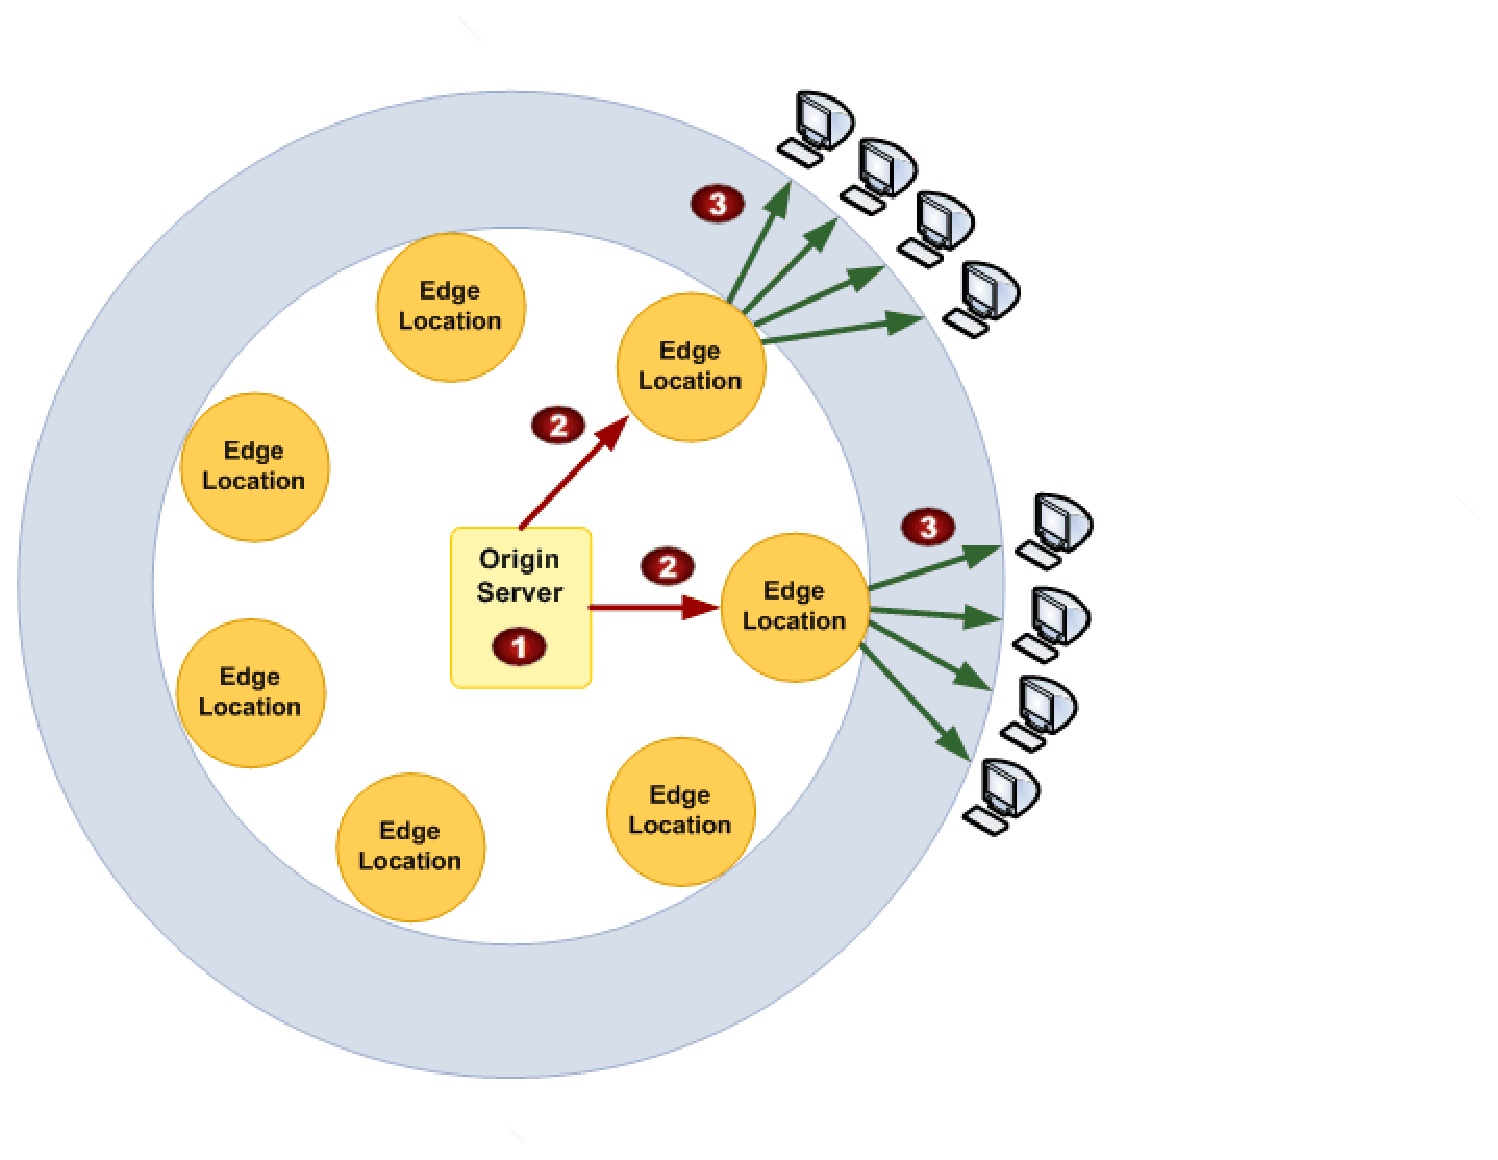
\includegraphics[width= 1.0 \textwidth]{cloudfront.eps}
\end{columns}
\end{frame}
%%%%%%%%%%%%%%%%%%%%%%%%%%%%%%%%%%%%%%%%%%%%%%%%%%%%%%%%%%%%%%%%%%%%%%%%%%%%%%
\subsection{Creating a CloudFront Distribution}
\begin{frame}[fragile]
\frametitle{Creating a CloudFront Distribution}

\begin{itemize}
\item Although it is possible to write code to create a CloudFront distribution for an S3
bucket, it’s easier to just use a graphical interface to create your distribution.
The AWS Management Console makes it very simple; select the Amazon
CloudFront tab and click the Create Distribution button

\item Create two CloudFront distributions associated with both origin and thumb image buckets. Once set up, you will have to wait several minutes while the CloudFront distribution is created
\item We will use CloudFront for efficient global distribution of the original and thumbnailed images

\end{itemize}

\end{frame}
%%%%%%%%%%%%%%%%%%%%%%%%%%%%%%%%%%%%%%%%%%%%%%%%%%%%%%%%%%%%%%%%%%%%%%%%%%%%%%

\subsection{Listing CloudFront Distributions}
\begin{frame}[fragile,allowframebreaks]
\frametitle{Listing CloudFront Distributions}
\begin{itemize}
\item Here is a simple script to list all of your CloudFront distributions

\lstset{language=Ruby, style=eclipse}
\begin{lstlisting}[escapechar=!]
#
# aws_app/s3/list_distributions.rb
#
# Usage: ruby list_distributions.rb
#

require File.expand_path(File.dirname(__FILE__) + '/../config')
require File.expand_path(File.dirname(__FILE__) + '/book.inc')

# get an instance of the CloudFront interface using the default configuration
cloud_front = AWS::CloudFront.new

# get the distributions
distributions = cloud_front.client.list_distributions

# for each distribution, print Id, domain name and origins
distributions[:items].each do |distribution|
  puts "Id = #{distribution[:id]}"
  puts "Domain name = #{distribution[:domain_name]}"
  puts "Origins = #{distribution[:origins]}"
end
\end{lstlisting}

\item Run \texttt{list\_distribution} utility
\lstset{language=shell}
\begin{lstlisting}[escapechar=!]
$  ruby s3/list_distributions.rb 
!\outputcommand{Id = EDXGI4G4HKW3B\\
Domain name = d1xhkx9ok8zmm7.cloudfront.net\\
\dots}!
\end{lstlisting} 
\end{itemize}
\end{frame}
%%%%%%%%%%%%%%%%%%%%%%%%%%%%%%%%%%%%%%%%%%%%%%%%%%%%%%%%%%%%%%%%%%%%%%%%%%%%%%
%%%%%%%%%%%%%%%%%%%%%%%%%%%%%%%%%%%%%%%%%%%%%%%%%%%%%%%%%%%%%%%%%%%%%%%%%%%%%%

\subsection{Listing S3 Files with Thumbnails with CloudFront}
\begin{frame}[fragile,allowframebreaks]
\frametitle{Listing S3 Files with Thumbnails with CloudFront}
\begin{itemize}
\item We first need one more utility function
to make this work: the  function that will return the
CloudFront distribution for a given S3 bucket. You guessed it, we’ll put this one in
our \texttt{book.inc.rb} file:

\lstset{language=Ruby, style=eclipse}
\begin{lstlisting}[escapechar=!]
#
# aws_app/book.inc.rb
#
# This file is required by some *.rb files
# It defines default constant value
# and some useful functions:
#
#  find_distribution_for_bucket cloud_front, bucket
!\vdots!
THUMB_SIZE = 200
THUMB_BUCKET_SUFFIX = '-thumbs'

def find_distribution_for_bucket cloud_front, bucket
  distributions = cloud_front.client.list_distributions

  distributions[:items].each do |distribution|
    distribution[:origins][:items].each do |item|
      return distribution if item[:domain_name] =~ /^#{bucket}.s3.amazonaws.com$/
    end
  end
end
\end{lstlisting}

\item This function accepts a CloudFront access object and the name of a bucket. It fetches
the list of CloudFront distributions and attempts to match each one to the supplied
bucket name. If a match is made, the distribution object is returned

\item The code below is an enhanced version of \texttt{list\_bucket\_objects\_page.rb}, as seen
earlier in this chaptre. It adds a thumbnail to the table for all the image objects in
the bucket that also have a corresponding image in the thumbnail bucket. It also
uses the CloudFront URL if available:

\lstset{language=Ruby, style=eclipse}
\begin{lstlisting}[escapechar=!]
#
# aws_app/s3/list_bucket_objects_page_thumbs.rb
#
# Usage: ruby list_bucket_objects_page_thumbs <BUCKET_NAME|-> <THUMB_BUCKET_NAME|->"
#

require File.expand_path(File.dirname(__FILE__) + '/../config')
require File.expand_path(File.dirname(__FILE__) + '/book.inc.rb')

def get_file_list( s3, cloud_front, bucket_name, thumb_bucket_name )
  distribution = find_distribution_for_bucket cloud_front, bucket_name
  url = distribution ?  "https://#{distribution[:domain_name]}" : "#{S3_AMAZONAWS_URL}/#{bucket_name}"

  thumb_distribution = find_distribution_for_bucket cloud_front, thumb_bucket_name
  thumb_url = if thumb_distribution then
                 "https://#{thumb_distribution[:domain_name]}"
               else
                 "#{S3_AMAZONAWS_URL}/#{thumb_bucket_name}"
               end
  
  # access to objects in the buckets
  objects = get_bucket_objects s3, bucket_name
  thumb_objects = get_bucket_objects s3, thumb_bucket_name

  file_list = []
  objects.each do |object|
    key = object[:key]
    thumb_uri = thumb_objects.detect{|thumb_object| thumb_object[:key] == key}?  "#{thumb_url}/#{key}": ''

    file_list << { key: key, size: object[:size], url: "#{url}/#{key}", thumb_url: thumb_uri}
    return file_list if file_list.size > 10
  end
  file_list
end

if __FILE__ == $0
  unless ARGV.size == 2
    puts "Usage: #{__FILE__} <BUCKET_NAME|-> <THUMB_BUCKET_NAME|->"
    exit 1
  end

  (bucket_name, thumb_bucket_name) = ARGV
  bucket_name = BOOK_BUCKET if bucket_name == '-'
  thumb_bucket_name = "#{BOOK_BUCKET}#{THUMB_BUCKET_SUFFIX}" if thumb_bucket_name == '-'

  # get an instance of the S3 interface using the default configuration
  s3 = AWS::S3.new

  # get an instance of the CloudFront interface using the default configuration
  cloud_front = AWS::CloudFront.new

  puts get_file_list( s3, cloud_front, bucket_name, thumb_bucket_name ).to_s
end
\end{lstlisting}

\item The template file \texttt{list\_bucket\_objects\_page\_thumbs.html.erb} code is
\lstset{language=Ruby, style=eclipse}
\begin{lstlisting}
<!DOCTYPE html>
<html>
<head>
  <title><%= @output_title %></title>
</head>
<body>
<div>
  <h1><%= @output_title %></h1>
  <p><%= @output_message %></p>
  <table>
    <thead>
    <tr><th>Thumb</th><th>File</th><th>Size</th></tr>
    </thead>
    <tbody>
    <% @file_list.each do |file| %>
        <tr>
          <td>
            <% if file[:thumb_url] != '' %>
                <a> <img src="<%= file[:thumb_url] %>"</a>
            <% end %>
          </td>
          <td><a href="<%= file[:url] %>"><%= file[:url] %></a></td>
          <td><%= file[:size] %></td>
        </tr>
    <% end %>
    </tbody>
  </table>
</div>
</body>
</html>
\end{lstlisting}

\item The code file \texttt{server.rb} for server is
\lstset{language=Ruby, style=eclipse}
\begin{lstlisting}[escapechar=!]
#
# aws_app/server.rb
#
require 'sinatra'
require File.expand_path("#{File.dirname(__FILE__)}/config")
require File.expand_path("#{File.dirname(__FILE__)}/s3/book.inc") !\circled{1}!

require File.expand_path("#{File.dirname(__FILE__)}/s3/list_bucket_objects_page_thumbs")

#  !\circled{2}!
routes = %w(/s3/list_buckets /s3/list_bucket_objects /s3/list_bucket_objects_page_thumbs)
routes.each do |route|
  get route do
    title = 'Expert in Virtualization and Cloud Computing'
    @s3 = AWS::S3.new
    case route
      when routes[0]
        @output_title = "#{title} - List of S3 buckets"
        @output_message = 'A simple HTML list of your S3 buckets'
      when routes[1]
        @bucket_name = params[:bucket_name].nil? ? BOOK_BUCKET : params[:bucket_name]
        @output_title = "#{title} - List of S3 objects in a bucket"
        @output_message = "A simple HTML table displaying of all the objects in the #{@bucket_name} bucket"
        @bucket_objects =  get_bucket_objects @s3, @bucket_name
      when routes[2] # !\circled{3}!
        @bucket_name = params[:bucket_name].nil? ? BOOK_BUCKET : params[:bucket_name]
        @thumb_bucket_name = "#{@bucket_name}#{THUMB_BUCKET_SUFFIX}"
        @output_title = "#{title} - List of S3 objects in a bucket with thumbnails (via CloudFront)"
        @output_message = "A simple HTML table displaying of all the objects in the #{@bucket_name} bucket"
        # get an instance of the CloudFront interface using the default configuration
        @cloud_front = AWS::CloudFront.new
        @file_list = get_file_list( @s3, @cloud_front, @bucket_name, @thumb_bucket_name )
        puts @file_list.to_s
    end
    erb :"#{route}.html"
  end
end

\end{lstlisting}

\item We curl \url{http://localhost:4567/s3/list\_bucket\_objects\_page\_thumbs} in order to check the written code
\end{itemize}
\end{frame}

\section{Homework}
\begin{frame}[fragile, allowframebreaks]
\frametitle{Homework}
\begin{itemize}
\item  S3 Filesystem (with Elastic Drive? witn s3fs?)
\item \texttt{s3 sync}
\begin{enumerate}
\item The following \texttt{sync} command syncs objects under a specified prefix and bucket to files in a local directory by uploading the local files to \acrshort{s3}. A local file will require uploading if the size of the local file is different than the size of the \acrshort{s3} object, the last modified time of the local file is newer than the last modified time of the \acrshort{s3} object, or the local file does not exist under the specified bucket and prefix. In this example, the user syncs the bucket mybucket to the local current directory. The local current directory contains the files \texttt{test.txt} and \texttt{test2.txt}. The bucket mybucket contains no objects

\lstset{language=shell}
\begin{lstlisting}[escapechar=!]
$ s3 sync . s3://mybucket
!\outputcommand{upload: test.txt to s3://mybucket/test.txt\\
upload: test2.txt to s3://mybucket/test2.txt}!
\end{lstlisting}

\item The following \texttt{sync} command syncs objects under a specified prefix and bucket to objects under another specified prefix and bucket by copying \acrshort{s3} objects. A \acrshort{s3} object will require copying if the sizes of the two \acrshort{s3} objects differ, the last modified time of the source is newer than the last modified time of the destination, or the \acrshort{s3} object does not exist under the specified bucket and prefix destination. In this example, the user syncs the bucket mybucket2 to the bucket mybucket. The bucket mybucket contains the objects \texttt{test.txt} and \texttt{test2.txt}. The bucket mybucket2 contains no objects

\lstset{language=shell}
\begin{lstlisting}[escapechar=!]
$ s3 sync s3://mybucket s3://mybucket2
!\outputcommand{
copy: s3://mybucket/test.txt to s3://mybucket2/test.txt\\
copy: s3://mybucket/test2.txt to s3://mybucket2/test2.txt}!
\end{lstlisting}


\item The following \texttt{sync} command syncs files in a local directory to objects under a specified prefix and bucket by downloading \acrshort{s3} objects. A \acrshort{s3} object will require downloading if the size of the \acrshort{s3} object differs from the size of the local file, the last modified time of the \acrshort{s3} object is older than the last modified time of the local file, or the \acrshort{s3} object does not exist in the local directory. Take note that when objects are downloaded from \acrshort{s3}, the last modified time of the local file is changed to the last modified time of the \acrshort{s3} object. In this example, the user syncs the current local directory to the bucket mybucket. The bucket mybucket contains the objects \texttt{test.txt} and \texttt{test2.txt}. The current local directory has no files

\lstset{language=shell}
\begin{lstlisting}[escapechar=!]
$ s3 sync s3://mybucket .
!\outputcommand{
download: s3://mybucket/test.txt to test.txt\\
download: s3://mybucket/test2.txt to test2.txt}!
\end{lstlisting}

\item The following \texttt{sync} command syncs objects under a specified prefix and bucket to files in a local directory by uploading the local files to \acrshort{s3}. Because the --delete parameter flag is thrown, any files existing under the specified prefix and bucket but not existing in the local directory will be deleted. In this example, the user syncs the bucket mybucket to the local current directory. The local current directory contains the files \texttt{test.txt} and \texttt{test2.txt}. The bucket mybucket contains the object \texttt{test3.txt}


\lstset{language=shell}
\begin{lstlisting}[escapechar=!]
$ s3 sync . s3://mybucket --delete
!\outputcommand{
upload: test.txt to s3://mybucket/test.txt\\
upload: test2.txt to s3://mybucket/test2.txt\\
delete: s3://mybucket/test3.txt}!
\end{lstlisting}

\item The following \texttt{sync} command syncs objects under a specified prefix and bucket to files in a local directory by uploading the local files to \acrshort{s3}. Because the --exclude parameter flag is thrown, all files matching the pattern existing both in \acrshort{s3} and locally will be excluded from the sync. In this example, the user syncs the bucket mybucket to the local current directory. The local current directory contains the files test.jpg and \texttt{test2.txt}. The bucket mybucket contains the object \texttt{test.jpg} of a different size than the local \texttt{test.jpg}.

\lstset{language=shell}
\begin{lstlisting}[escapechar=!]
$ s3 sync . s3://mybucket --exclude "*.jpg"
!\outputcommand{
upload: test2.txt to s3://mybucket/test2.txt}!
\end{lstlisting}

\item The following \texttt{sync} command syncs files under a local directory to objects under a specified prefix and bucket by downloading the local files to \acrshort{s3}. This example uses the --exclude parameter flag to exclude a specified directory and \acrshort{s3} prefix from the sync command. In this example, the user syncs the local current directory to the bucket mybucket. The local current directory contains the files \texttt{test.txt} and another/\texttt{test2.txt}. The bucket mybucket contains the object another/\texttt{test5.txt}.

\lstset{language=shell}
\begin{lstlisting}[escapechar=!]
$ s3 sync s3://mybucket/ . --exclude "*another/*"
!\outputcommand{
download: s3://mybucket/test1.txt to test1.txt}!
\end{lstlisting}
\end{enumerate}
\end{itemize}

\end{frame}

%%%%%%%%%%%%%%%%%%%%%%%%%%%%%%%%%%%%%%%%%%%%%%%%%%%%%%%%%%%%%%%%%%%%%%%%%%%%%%
\end{document}

